%                                             -*- coding: utf-8 -*-
% Mindenkinek csak javasolni tudjuk, hogy latex-et használjon.
% Szakdolgozatnál vagy diplománál már egyértelműen kijönnek az
% előnyei a Worddel szemben.  Ennek ellenére ez a sablon messze nem
% tökéletes.  Ha valamit javítanál benne, kérlek, küld vissza, hogy
% hallgatótársaid is profitáljanak belőle.  Köszönöm.

% További nehézséget okoz, hogy a népszerű latex disztribúciók nem
% tartalmazzák a legújabb változatát a magyar.ldf-nek.  A szükséges
% fájlokat a sablon mellé bemásoltuk, de le is tölthetőek innen:
% http://www.math.bme.hu/latex/
%
%
%
\documentclass[a4paper,oneside]{article}
\usepackage[margin=3cm]{geometry}
% =================================================================
% Magyar nyelvi támogatás
%------------------------
% ###################
% Nyelvváltó parancsok:
%\selectlanguage{english}
%\selectlanguage{magyar}
% rövid angol beszúrás:  \foreignlanguage{english}{some english text}
% határozott névelők generálása ``magyar'' babel-el:
% argumentum+megfelelő határozott nevelő: \az{},\Az{}
% csak a megfelelő határozott nevelő: \az*{}, \Az*{}
% címkék: \aref{}, \aref*{}, képletekhez \aref()
%        \Aref{}, \Aref*{}, képletekhez \Aref()
% oldalak: \apageref{}, \apageref*{}
%        \Apageref{}, \Apageref*{}
% idézetek: \acite, \acite*, \Acite, \Acite*
% ###################
\usepackage[english,magyar]{babel} %vegyes nyelvi támogatás a
% magyar helyesírás ellenőrzéshez (ispell) és elválasztáshoz
\selectlanguage{magyar}

%=================================================================
% direkt ékezetes karakter beírás támogatás
%-------------------------------------------
\usepackage[T1]{fontenc}
\usepackage[utf8]{inputenc}
\usepackage{multirow} 
%================================================================
% Undorító dolog bitmappelt (Type III) betűtípust nézni a PDF-ben
% képernyőn. Az alapértelmezett Computer Modern font LaTex-ben
% bitmappelt, ezért használjunk Times fontot:
\usepackage{times}
\usepackage{syntax}
\usepackage{amsmath}
\usepackage{listings}
\usepackage{xcolor}
\usepackage{xspace}
\usepackage{caption}
\usepackage{tikz}
\usetikzlibrary{positioning, arrows.meta, fit, backgrounds, calc}

% Rust-specifikus színek definiálása (VS Code / modern IDE stílus)
\definecolor{rustkeyword}{rgb}{0.0, 0.0, 0.8}
\definecolor{rusttype}{rgb}{0.17, 0.57, 0.68}
\definecolor{rustcomment}{rgb}{0.0, 0.5, 0.0}
\definecolor{ruststring}{rgb}{0.64, 0.08, 0.08}
\definecolor{backcolour}{rgb}{0.98, 0.98, 0.96}

% Saját Rust nyelv definíciója a listings számára
\lstdefinelanguage{Rust}{
    keywords={fn, let, mut, match, return, if, else, pub, crate, impl, enum, struct, use, type, for, while, loop, break, continue, ref},
    keywordstyle=\color{rustkeyword}\bfseries,
    ndkeywords={Result, ReductionState, NodeComb, Node, ArrayVec, EngineError},
    ndkeywordstyle=\color{rusttype}\bfseries,
    sensitive=true,
    comment=[l]{//},
    morecomment=[s]{/*}{*/},
    commentstyle=\color{rustcomment}\itshape,
    string=[b]",
    stringstyle=\color{ruststring},
    morestring=[b]',
}

\lstdefinestyle{ruststyle}{
    language=Rust,
    backgroundcolor=\color{backcolour},   
    basicstyle=\ttfamily\footnotesize,
    breakatwhitespace=false,         
    breaklines=true,                 
    captionpos=b,                    
    keepspaces=true,                 
    numbers=left,                    
    numbersep=5pt,                  
    numberstyle=\tiny\color{gray},
    showspaces=false,                
    showstringspaces=false,
    showtabs=false,                  
    tabsize=4,
    frame=single,
    rulecolor=\color{black!20}
}

\lstset{style=ruststyle}
\renewcommand{\lstlistingname}{Kódrészlet}

%================================================================
% ha ábrát akarunk beemelni, akkor használjuk a graphicx/graphics
% csomagot és az \includegraphics[width=<width>]{abra.pdf} parancsot
\usepackage{graphicx} %for graphics
%kepek helye a gyokerhez(ehhez a file-hoz kepest) kepest
\graphicspath{{./figs/}}

%================================================================
% Kötelezően használjuk a hyperref csomagot, mert ezzel többek között 
%  kultúrált hyperlinkelt PDF-et lehet csinálni az alábbi
%  variációkban, különféle hyperref backend-ekkel:
%  pdflatex,dvipdfm,ps2pdf
% tapsztalataim szerint a MikTeX (Win32) a 'dvipdfm' konverzióval
% optimális  míg a teTeX (Linux/Solaris) jobb szereti a 'dvips' módszert
%------------------------------------
% pontosan egyet kommentezzünk be!!!!!!!
% értelemszerűen backend függően generáljunk dvi-ból PDF-et!!!
%------------------------------------
% A hyperref csomag az utolsó beolvasott csomag legyen, kivéve néhány
% problémás csomagot, pl. algorithm
%-----------
% ########################### FONTOS ###########################
% A hyperref hibásan működik a babel csomag 'magyar.ldf' fájljának
% 1.5-ös verziójánál korábbi változatával. 2004. februárjában a MikTeX
% és teTex disztribúciók még csak a v.1.4 verziót tartalmazták! A fájl
% aktuális verziója a BME Matematikai intézet LaTeX honlapjáról
% elérhető: http://www.math.bme.hu/latex/ 
% A lusták kedvéért a jelen sablon mellé is mellékelem:
% magyarlatex_0.01-2.tar.gz 
% ########################### FONTOS ###########################
%-----------
\usepackage[colorlinks=true]{hyperref}

%%%%%%%%%%%%%%%%%%%%%%%%%%%%%%%%%%%%%%%%%%%%%%%%%%%%%%%%%%%%%%%%%%%
% Itt kezdődik maga a dokumentum
%%%%%%%%%%%%%%%%%%%%%%%%%%%%%%%%%%%%%%%%%%%%%%%%%%%%%%%%%%%%%%%%%%
\begin{document}
\input{onlabmacros} % Ez kell!!!
% $\lambda$
\newcommand{\lam}{\ensuremath{\lambda}}

% SKI
\newcommand{\ski}{\textsf{SKI}}
\newcommand{\Icomb}{\textsf{I}}
\newcommand{\Kcomb}{\textsf{K}}
\newcommand{\Scomb}{\textsf{S}}
\newcommand{\Ccomb}{\textsf{C}}
\newcommand{\Bcomb}{\textsf{B}}
\markright{Orbán Levente (CZ6NDB)} % egyoldalas fejléc!!!
%--------------------------------------------------------------------
% fedlap
%--------------------------------------------------------------------
\begin{titlepage}
  %bme logo 
  \begin{figure}[h]
    \centering
    
\includegraphics[width=12cm]{bme-logo}
    \label{fig:bme-logo}
  \end{figure}
  \thispagestyle{empty}
  %cím generálás
  \onlabcim

  % \begin{center}
  %   \begin{tabular}{ p{3cm} p{5cm} }

  %   Készítette: & Beszámoló Péter  \\
  %   Neptun-kód: & BPOX43  \\
  %   Ágazat: & Médiainformatika  \\
  %   E-mail cím: & b.peter@onlab.hu  \\
  %   Konzulens: & Dr. Péhádes István  \\
  %   E-mail cím: & pehades@tmit.bme.hu  \\
  %   Konzulens: & Doktor Andusz  \\
  %   E-mail cím: & doktora@tmit.bme.hu  \\

  %   \end{tabular}
  % \end{center}


  %\szerzo argumentumok: #1=Név, #2=Neptunkód, #3=szakirány, #4=email,#5 konzulens-1, #6 konzulens-1-email, #7 konzulens-2, #8 konzulens-2-email
  \onlabszerzo{Orbán Levente}{CZ6NDB}{Szoftverfejlesztés}{orban.levente.laszlo@gmail.com}{Németh Gábor}{nemethgab@tmit.bme.hu}{}{}

  %\feladatcim argumentuma a feladat rövid, 1 soros címe
  \feladatcim{Interaktív SKI-kombinátor kalkulus fordító és vizualizáló}

  %\feladatmaga argumentuma a feladat 1-2 bekezdésnyi ismertetése
  \feladatmaga{A hallgató feladata egy webes eszköz (Combinator Explorer) elkészítése, amely SKI-kifejezések esetén megmutatja a redukciós lépéseket, vizualizálja a redexeket, és felrajzolja a kiértékelési fát. A redukció során többféle kiértékelési stratégiát támogat, valamint az SKI-kifejezéseket lefordítja \lam-kalkulusba. Az eszköz hidat képez a formális elmélet és a gyakorlati megvalósítás között: oktatási segédeszköz, amely mélyíti a funkcionális programozás, illetve a fordítóprogramok működésének megértését.}

  %\tanevfelev argumentumok:
  % #1=Tanév (xxxx/xx alakban), #2=félév (pont nélkül!)

  \tanevfelev{2025/26}{II}

\end{titlepage}

%==================================================================
\section{A laboratóriumi munka környezetének ismertetése,
  a munka előzményei és kiindulási állapota}
\label{sec:kornyezet}
% A munka  előzményei és kiindulási állapota
% \newpage
\subsection{Bevezető}
\label{sec:bevezeto}

Az elmúlt három évtizedben egyre nagyobb jelentőségre tett szert a funkcionális programozás az iteratív és objektumorientált paradigmákkal szemben. Az figyelhető meg, hogy azok a programozási nyelvek, amelyek tradicionálisan objektumorientált szemléletűek voltak (például C++, Java) napjainkra jelentős számú funkcionális elemmel bővültek (anonim függvények, lista komprehenzió, magasabb rendű függvények, stb.). Továbbá azok a nyelvek, amelyek az elmúlt évtizedben tettek szert népszerűségre (például Rust) már a kezdetektől fogva egy több paradigmát ötvöző nézettel lettek tervezve. Ezeket az új eszközöket viszont -- mind a már piacon lévő mérnökök továbbképzése, mind a felsőoktatásban résztvevők oktatása szempontjából -- pedagógiailag még a mai napig nehéz kielégítően oktatni. A funkcionális paradigma -- illetve annak a matematikai alapjai -- idegenek lehetnek a mérnöki beállítottságú közönség számára.

A jelen írásos beszámolómban bemutatott szoftver ezt a pedagógiai hiányt próbálja pótolni: egy olyan vizuális, interaktív, webes eszközt ad a pedagógusok kezébe, amellyel a funkcionális programozást egészen a matematikai alapokig visszamenően lehet hatékonyabban oktatni, hozzá pontosabb intuíciót építeni.

A választott megközelítés (vizuális, webes program) nem egyedi. Számtalan más olyan témakörhöz, amelyek tradicionálisan pedagógiai kihívásokat jelentettek (generált gépi kód, vagy reguláris kifejezések elemzése) készült hasonló alapötletekkel rendelkező szoftver (mint például a Compiler Explorer \cite{godboltCompilerExplorer}, vagy Regex101 \cite{dibRegex101BuildTest}).

A jelen beszámolómban bemutatott megközelítés a modern funkcionális nyelvek matematikai alapjait kívánja megcélozni (többek között redukciós láncok és gráfok, kiértékelési sorrendek, \lam- és \ski-kalkulus). Ezen alaptudás ismeretében a legtöbb modern funkcionális nyelv (ML-család, Lisp-család) szemantikáinak a működése -- legalábbis magas szinten -- könnyebben elsajátítható.

\subsection{Elméleti összefoglaló}

\subsubsection{\texorpdfstring{\lam}{lambda}-kalkulus}
A modern funkcionális programozási nyelvek alapjaikban a (típus nélküli) \lam-kalkulusra építenek\footnote{Tekinthetőek a \lam-kalkulus kibővített, változatának (legyen szó típusokról, vagy \textsf{let}-kötésekről, etc.). Példa erre az ML-család (Standard ML, Caml, Haskell), amelyek közelítőleg felfoghatóak úgy, mint a \lam-kalkulus polimorf Hindley-Milner típusrendszerrel való kiegészítése.}, amely egy általános célú, Turing-teljes programozási nyelv. Az egyik legegyszerűbb Turing-teljes nyelv, hiszen csak három konstrukcióra épít (lambda-kifejezések, lambda-absztrakciók, és applikációk). A \lam-kalkulus nyelvtanának formális definíciója \aref{fig:lambda-grammar}.~ábrán látható.

\begin{figure}[htbp]
  \centering
  \begin{minipage}{7.5cm}
    \setlength{\grammarindent}{9em}

    \begin{grammar}
      <\lam-kifejezés> ::= <változó>
      \alt <\lam-absztrakció>
      \alt <applikáció>

      <\lam-absztrakció> ::= `\lam' <változó> `.' <\lam-kifejezés>

      <applikáció> ::= <\lam-kifejezés> <\lam-kifejezés>
    \end{grammar}
  \end{minipage}
  \caption{A \lam-kalkulus szintaktikája}
  \label{fig:lambda-grammar}
\end{figure}

A \lam-absztrakció segítségével tudunk függvényeket definiálni, amelyeknek paramétereket az applikáció konstrukciójával tudunk adni. Ha kicsit módosítjuk a nyelvtanunkat, hogy szám konstansokat, és egyéb kényelmes konstrukciókat megengedjen, akkor írhatjuk például:

\[
  \begin{aligned}
     & \lambda x.(5*x)      \\
     & (\lambda x.(5*x))(3) \\
     & 15
  \end{aligned}
\]

Az első sorban definiálunk egy függvényt, amely ötszörözi a bemenetét. A második sorban meghívjuk ezt a függvényt a $3$ bemenettel. Az utolsó sorban a szorzás eredménye látható. Fontos megjegyezni, hogy az applikáció bal-asszociatív \cite{pierceTypesProgrammingLanguages2002a}.

\subsubsection{Az \ski-kalkulus}
\label{sec:a-ski-kalkulus-def}

A kombinátorok absztrakt matematikai konstrukciók, viszont megértésük és történelmi hátterük kritikus fontosságú a modern számítástudomány, különösen a funkcionális programozás, vagy a kiszámíthatóság modelljeinek vizsgálatához.

Általánosságban különböző problémák formális, szimbolikus ábrázolását már az ókorban megkísérelték. Így született Arisztotelész logikája és Euklidész geometriája. A számítástudomány szempontjából viszont a 19. században a Boole-algebra megjelenése jelentette a legnagyobb áttörést. A 20. század fordulóján a matematikusok arra tettek kísérletet, hogy a teljes matematikát egy szigorú, tiszta logikai alapra helyezzék. Ahogy ezek a logikai keretrendszerek egyre nagyobbak lettek, megjelent az igény a bizonyos axiómák meghatározására. Ennek a törekvésnek a legismertebb példája a Sheffer-vonás felfedezése, amely bebizonyította, hogy a teljes ítéletkalkulus felépíthető egyetlen logikai kapu segítségével (NAND) \cite{shefferSetFiveIndependent1913}. Felmerült a kérdés: ha a logikai axiómák ilyen elemi szintre redukálhatóak, megtehető-e ugyanez általánosságban a függvényekkel és a változókkal is \cite{pierceTypesProgrammingLanguages2002a}?

Moses Schönfinkel 1920-ban pontosan erre tett kísérletet \cite{schoenfinkelUeberBausteineMathematischen1924}. Felismerte, hogy ha a függvényeket kellőképpen általánosítjuk (egy függvény egy másik függvényt is kaphat paraméterként, és visszatérési értéke is lehet egy függvény), a változók feleslegessé válnak. Ezzel az elképzeléssel lefektette a kombinátorkalkulus  alapjait. A kombinátorkalkulus leghíresebb és leginkább letisztult\footnote{Bár a fent említett \ski rendszer az általánosan vizsgált forma, fontos megemlíteni, hogy léteznek kevesebb kombinátorokat igénybe vevő, Turing-teljes rendszerek is. Ilyen például az \Scomb és \Kcomb kombinátorokból álló bázis. Ez abból adódik, hogy az \Icomb kombinátor kifejezhető a másik kettőből, például \(\left(\Scomb\Kcomb\Kcomb\right)\) módon.} formalizációja az \ski-kalkulus, amelyet Schönfinkel munkássága nyomán Haskell Curry dolgozott ki \cite{curryGrundlagenKombinatorischenLogik1930}. Ez pusztán három előre definiált kombinátor egymás utáni alkalmazásával is képes Turing-teljes számítások leírására.

A rendszer a következő három kombinátorból áll:
\begin{itemize}
  \item Az egyváltozós identitás kombinátor (\Icomb), amely beavatkozás nélkül, egyszerűen visszaadja a kapott argumentumát.
  \item A kétváltozós konstans kombinátor (\Kcomb), amely olyan függvényt állít elő, ami a második argumentumát mindig figyelmen kívül hagyja, és visszaadja az elsőt.
  \item A háromváltozós szubsztitúciós kombinátor (\Scomb), amely az argumentumok szétosztását és a függvényalkalmazás láncolatát végzi.
\end{itemize}

Bár a rendszert általában további kombinátorokkal is ki szokás egészíteni a kényelmesség és átláthatóság érdekében, ezek mind levezethetőek a fenti három kombinátorból.

Ha a \lam-kalkulus, és az \ski-kalkulus és Turing-teljesek, akkor bizonyára kell lennie valamilyen ekvivalenciának közöttük. Alább megadom az \ski-kalkulus három kombinátorának a \lam-kalkulus szerinti definícióját:

\[
  \begin{aligned}
    \Icomb & = \lambda x.x                              \\
    \Kcomb & = \lambda x.(\lambda y.x)                  \\
    \Scomb & = \lambda x.(\lambda y.(\lambda z.xz(yz)))
  \end{aligned}
\]

Ezeknek a szabályoknak az alkalmazásával tetszőleges \ski-kalkulus kifejezést át lehet alakítani \lam-kalkulus kifejezéssé, melyre a programban lehetőség is van.

\subsection{A munka állapota, készültségi foka a félév elején}
\label{sec:munka-allap-kesz}

A jelen félév előtti szünetben már elkezdtem feldolgozni a témához releváns irodalmat. A 2025/26/I. félévben egy olyan tárgyat hallgattam, amelyben jelentős szerepe volt a \lam-kalkulusnak, kategória elméletnek. Ezek az előadások nagyban hozzájárultak az előzetes tudás megszerzéséhez. A konzulensem számos releváns könyvet ajánlott feldolgozásra, többek között Smullyan \cite{smullyanMockMockingbirdOther2000} és Wolfram \cite{wolframCombinatorsCentennialView2020, wolframCombinatorsStoryComputation2020} írásait.

%==================================================================
\section{Az elvégzett munka és az eredmények ismertetése}
\label{sec:az-elvegzett-munka}

\subsection{Az architektúra megtervezése}
\label{sec:az-arch-megterv}

A program megtervezése során fontos cél volt annak modális felépítése
és úgynevezett \emph{\foreignlanguage{english}{Separation of Concerns}} elve \cite{readeElementsFunctionalProgramming1989}. Ennek megfelelően az elkészült program két jól elkülönülő részre bomlik: frontendre és backendre. Míg a frontend felelős a felhasználóval való kommunikációért, illetve az eredmények megjelenítésért, addig a backend végzi a tényleges számítási feladatot.

A frontend és a backend közötti tiszta kommunikáció megteremtésére
a homlokzat (facade) mintát \cite{gammaDesignPatternsElements1995} alkalmaztam. Ez az API réteg (\texttt{lexor-api}) elrejti a backend komplexitását,
és egy könnyen használható interfészt biztosít a frontend számára
(az architektúra egyszerűsített vizuális modellje \aref{fig:tikz-arch}.~ábrán látható).

\begin{figure}[htbp]
  \centering
  \scalebox{0.75}{
    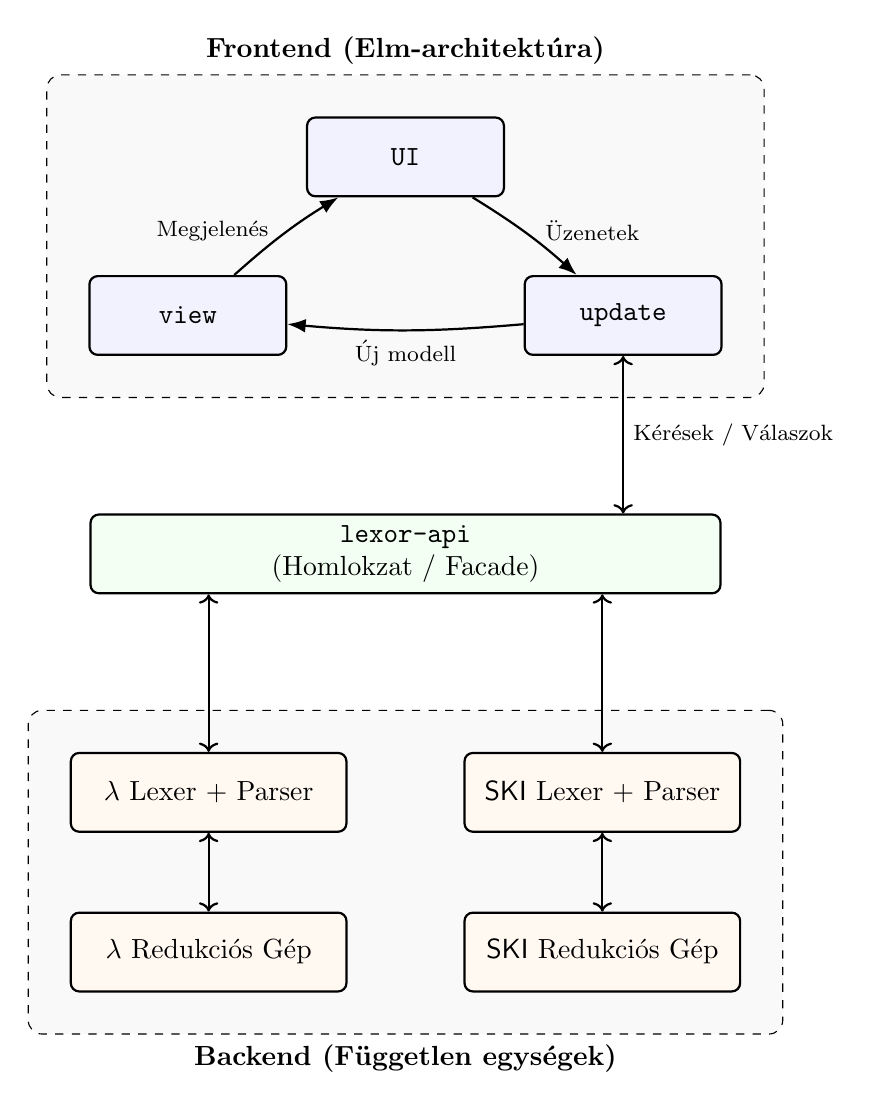
\begin{tikzpicture}[
        node distance = 1.5cm and 2cm,
        box/.style = {draw, rectangle, minimum width=2.5cm, minimum height=1cm, align=center, fill=blue!5, rounded corners=3pt, thick},
        api/.style = {draw, rectangle, minimum width=8cm, minimum height=1cm, align=center, fill=green!5, rounded corners=3pt, thick},
        backend/.style = {draw, rectangle, minimum width=3.5cm, minimum height=1cm, align=center, fill=orange!5, rounded corners=3pt, thick},
        arrow/.style = {-Latex, thick},
        group/.style = {draw, rectangle, dashed, inner sep=15pt, fill=gray!5, rounded corners=5pt}
      ]

      % ================= FRONTEND =================
      \node[box] (update) {\texttt{update}};
      \node[box, left=3cm of update] (view) {\texttt{view}};
      \node[box, above=1.5cm of $(view)!0.5!(update)$] (userint) {\texttt{UI}};

      % Frontend nyilak (Elm körforgás)
      \draw[arrow] (view) to[bend left=5] node[left, font=\footnotesize, xshift=-2pt, yshift=+1pt] {Megjelenés} (userint);
      \draw[arrow] (update) to[bend left=5] node[below, font=\footnotesize] {Új modell} (view);
      \draw[arrow] (userint) to[bend left=5] node[right, font=\footnotesize, xshift=+3pt, yshift=+1pt] {Üzenetek} (update);

      % ================= API RÉTEG =================
      \coordinate (api-pos) at ($(view.south)!0.5!(update.south) - (0, 2cm)$);
      \node[api, anchor=north] (api) at (api-pos) {\texttt{lexor-api} \\ (Homlokzat / Facade)};

      % Kommunikáció Frontend és API között
      \draw[arrow, <->] (update.south) -- (update.south |- api.north) node[midway, right, font=\footnotesize] {Kérések / Válaszok};

      % ================= BACKEND =================
      % Lambda egység
      \node[backend, below=2cm of api, xshift=-2.5cm] (lam-parser) {$\lambda$ Lexer + Parser};
      \node[backend, below=1cm of lam-parser] (lam-engine) {$\lambda$ Redukciós Gép};
      \draw[arrow, <->] (lam-parser) -- (lam-engine);

      % SKI egység
      \node[backend, below=2cm of api, xshift=2.5cm] (ski-parser) {\textsf{SKI} Lexer + Parser};
      \node[backend, below=1cm of ski-parser] (ski-engine) {\textsf{SKI} Redukciós Gép};
      \draw[arrow, <->] (ski-parser) -- (ski-engine);

      % Kommunikáció API és Backend között
      \draw[arrow, <->] (api.south -| lam-parser.north) -- (lam-parser.north);
      \draw[arrow, <->] (api.south -| ski-parser.north) -- (ski-parser.north);

      % ================= HÁTTÉR DOBOZOK =================
      \begin{scope}[on background layer]
        % Frontend keret
        \node[group, fit=(view)(update)(userint), label={[font=\bfseries]above:Frontend (Elm-architektúra)}] (fe-group) {};

        % Backend keret
        \node[group, fit=(lam-parser)(lam-engine)(ski-parser)(ski-engine), label={[font=\bfseries]below:Backend (Független egységek)}] (be-group) {};
      \end{scope}

    \end{tikzpicture}
  }
  \captionsetup{justification=centering}
  \caption{Az alkalmazás rétegei és architektúrája}
  \label{fig:tikz-arch}
\end{figure}

A backend megtervezése során a fordítóprogramokból merítettem inspirációt \cite{EngineeringCompiler2023}. Így a backend is további két részből áll, ún. compiler frontendből és compiler backendből, amelyek közötti kommunikáció egy absztrakt adatstruktórán, a köztes reprezentáción keresztül történik. Ez a struktúra direkt azzal a megfontolással lett kialakítva, hogy a compiler backend még optimalizációkat fog végezni rajta, a felhasználó nem interaktál vele. Ilyen például \aref{sec:a-lam-kalkulus-impl}~fejezetben tárgyalt de Bruijn forma is.

A compiler frontend tartalmazza a lexert és a parsert. A nyelvtanok egyszerűsége miatt ezt a két elemet egy egységbe összevontam. A
compiler backend két redukciós gépet tartalmaz: egyet, ami \lam-kalkuluson, egyet, ami \ski-kalkuluson operál.

A frontend terén az úgynevezett \emph{Elm-architektúrát} \cite{elmArchitectureGuide} követtem, amely egy üzenetsor-alapú architektúra. Ez a megközelítés három részre bontja a frontendet:
\begin{itemize}
  \item A kezdeti \texttt{model}-re, amely az applikáció állapotát írja le. Ez az állapot nem mutábilis, tehát ahogy a felhasználó interakcióba lép vele, mindig egy teljesen új állapot jön létre.
  \item A \texttt{view} függvényre, amely a modell megjelenését írja le. A felhasználói interakciókat itt alakítom át üzenetekké.
  \item Az \texttt{update} függvényre, amely az üzenetsort kiolvasva végrehajtja a felhasználó összes parancsát a jelenlegi modellen, ezáltal egy új modellt létrehozva.
\end{itemize}
Ahogy a felhasználó interakcióba lép a felhasználói felülettel, úgy új üzenetek kerülnek az üzenetsorba. Az üzenetsort minden frame végén az \texttt{update} függvény kiüríti, és a tartalmát végrehajtja. Ezáltal egy új modell jön létre, amit átad a \texttt{view} függvénynek, ami egy új \texttt{UI}-t hoz létre.

\subsection{Redukciós gépek}
\label{sec:a-redukcios-gepek-impl}

\subsubsection{Az \ski-kalkulus}
\label{sec:a-ski-kalkulus-impl}

A redukciós gépek implementálásához a \foreignlanguage{english}{Graph Reduction Machine} (\foreignlanguage{english}{G-machine}) koncepcióját vizsgáltam meg. Optimalizálási célból a fa-alapú kiértékelés mellett az alkifejezések megosztása mellett döntöttem, amellyel exponenciálisan kevesebb lépésszámot vesznek igénybe az egyes redukciók \cite{LambdaNotFour}. Az elterjedtebb "sztringredukció" -- azaz amikor a bemenetet szövegmanipulációs módszerekkel alakítjuk át a redukciós szabályoknak megfelelően -- nem skálázódik elég jól hosszabb kifejezések kiértékelésére, illetve az előbb említett alkifejezés-megosztás technikáját sem tudom érvényesíteni.

A követelmények elemzése és a belső reprezentáció kialakítása után implementáltam egy \foreignlanguage{english}{G-machine}-t mind a \lam-kalkulus, mind az \ski-kalkulus esetében. Az ilyen redukciós gépek implementálása során gyakran használt, fa alapú AST (\foreignlanguage{english}{Abstract Syntax Tree}, absztrakt szintaxis fa) sokszor memóriatöredezettséghez és lassabb futáshoz vezethet. Ennek elkerülése érdekében a \foreignlanguage{english}{Flat-AST} (laposított AST) reprezentációs technikát használtam, amelyet egy aréna alapú memória-allokátorral párosítottam \cite{FlatteningASTsOther}. Egy rekurzív, fa alapú megközelítés lehet \aref{lst:rec-node-ast}.~kódrészletben bemutatott modell.
\begin{lstlisting}[float=htbp, caption={Egy rekurzív, mutató alapú gráf struktúra}, label={lst:rec-node-ast}]
enum NodeRec {
    S, K, I,
    App(Box<Self>, Box<Self>),
    Indirection(Box<Self>),
}
\end{lstlisting}
Itt pointereket tárolunk el a többi csúcsra, amely csökkentheti a memória lokalitását, illetve az adatstruktúra méretét is növelheti $64$-bites rendszereken. Ehhez képest az aréna allokátoros megközelítés -- melyet \aref{lst:arena-node-ast}.~kódrészlet mutat be -- nem használ mutatókat. Minden csúcsra az indexe alapján lehet hivatkozni, mely alapján az arénából kinyerhető. Így a különböző kifejezések akár teljesen szomszédos memóriarégiókban lehetnek, növelve a cache-kihasználtságot.
\begin{lstlisting}[float=htbp, caption={Egy aréna allokátoros gráf struktúra}, label={lst:arena-node-ast}]
enum NodeFlat {
    S, K, I,
    App(NodeIdx, NodeIdx),
    Indirection(NodeIdx),
}
\end{lstlisting}

A \foreignlanguage{english}{G-machine} a kombinátorok redukcióját egy állapotgép segítségével végzi. A kiértékelés során először végighaladunk a kifejezés "gerincén", amely azokból a csúcsokból áll, amit úgy kapunk, ha a fa gyökerétől kezdve addig megyünk balra, ameddig van baloldali gyerek. A gerincen összegyűlt csúcsok argumentumait a redukciós gép a megfelelő kombinátor szabályai szerint helyettesíti be (például az \Scomb, \Kcomb, \Icomb kombinátorok esetében).

Mivel a szoftver célja az oktatás megkönnyítése, több redukciós stratégiát is támogatnom kellett (például \foreignlanguage{english}{normal order}, \foreignlanguage{english}{call--by--value}). Ezek megértéséhez elemezzük \aref{fig:strategy}.~ábrát \cite{wolframCombinatorsCentennialView2020}, amely az alábbi kombinátor AST-ét ábrázolja:

\[
  \Scomb(\Scomb(\Scomb)(\Scomb)(\Scomb(\Scomb)(\Kcomb(\Kcomb)(\Scomb))(\Scomb)))(\Scomb)(\Scomb)(\Scomb(\Kcomb(\Scomb)(\Kcomb))(\Kcomb)(\Scomb))
\]

Az ábrán látható fában a szürke belső csomópontok az applikációkat (függvényalkalmazásokat) jelölik, a levelek pedig az egyes kombinátorokat. Látható, hogy egy ilyen komplex kifejezés esetén egyszerre több ponton is elvégezhető lenne a redukció. A támogatott stratégiák pontosan abban térnek el, hogy ezek közül melyiket választják:

\begin{itemize}
  \item Normál sorrend (\foreignlanguage{english}{normal order} és \foreignlanguage{english}{call--by--name}): Mindig a legbaloldalibb, legkülső (\foreignlanguage{english}{leftmost--outermost}) redukálható kifejezéseket (redexeket) választják ki. A gráfban ez a gyökértől balra haladva a legmagasabban fekvő kiemelt csomópont. A két stratégia között az a fő különbség, hogy míg a \foreignlanguage{english}{normal order} egy nem applikált függvény törzsén belül is elvégzi a redukciós lépéseket, addig a \foreignlanguage{english}{call--by--name} nem tesz ilyet, hanem megáll amint elér egy telítetlen absztrakciót (amelynek nincsen elég argumentuma ahhoz, hogy kiértékeljük). Ez utóbbi emiatt az úgynevezett gyenge fej-normálforma (\foreignlanguage{english}{weak head normal form}) \cite{Lambdakalkulus2007} állapotba hozza a kifejezéseket, ahol nincsen arra garancia, hogy az argumentumok között még nincsen kiértékelhető alkifejezés. A \foreignlanguage{english}{normal order} esetén normálformába kerülnek a kifejezések, amit már nem lehet tovább egyszerűsíteni \cite{pierceTypesProgrammingLanguages2002a}. Ez a két stratégia a redukálást \aref{fig:strategy}.~ábrán a $\Scomb(\Scomb(\Scomb)(\Scomb)(\Scomb(\Scomb)(\Kcomb(\Kcomb)(\Scomb))(\Scomb)))(\Scomb)(\Scomb)$ alkifejezéssel kezdené.
  \item Applikatív sorrend (\foreignlanguage{english}{applicative order} és \foreignlanguage{english}{call--by--value}): A legbaloldalibb, legbelső (\foreignlanguage{english}{leftmost--innermost}) redexet redukálják először. Hasonló különbség létezik ezen két stratégia között is: a \foreignlanguage{english}{call--by--value} nem végez kiértékelést az absztrakciók törzsén belül, míg az \foreignlanguage{english}{applicative order} igen. A gyakorlatban ezek abban térnek el az előző pontban említett stratégiáktól, hogy egy függvény alkalmazása előtt -- amennyiben annak minden paramétere rendelkezésre áll -- az argumentumait értékeli ki, a fában lentről felfelé haladva. Ez a két stratégia a kiértékelést \aref{fig:strategy}.~ábrán a $\Kcomb(\Kcomb)(\Scomb)$ alkifejezéssel kezdené. A legtöbb modern imperatív és szigorú nyelv (pl. C++, Rust, OCaml) ezt használja.
\end{itemize}

A stratégiák megválasztása azért kiemelten fontos, mert vannak olyan \ski-kalkulus kifejezések, amelyeknek a redukciója bizonyos stratégiákat alkalmazva végtelen ciklusba kerül. Tekintsük például az alábbi kifejezést:

\[
  \Kcomb\Icomb((\Scomb\Icomb\Icomb)(\Scomb\Icomb\Icomb))
\]

Applikatív sorrend alkalmazásával, a gép először megpróbálja az argumentumokat ($(\Scomb\Icomb\Icomb)(\Scomb\Icomb\Icomb)$) teljesen kiértékelni, mielőtt a $\Kcomb$ kombinátort alkalmazná. Ez egy végtelen ciklust eredményez. Normál sorrend szerint viszont az algoritmus a legkülső redexet (a $\Kcomb$ applikációját) választja ki először, ezáltal a második argumentum (a divergáló kifejezés) eltűnik, és a kifejezés normál-formába kerül ($\Icomb$).

A kialakításban különösen figyeltem arra, hogy a redukciós logika moduláris maradjon, így az egyes stratégiák könnyen cserélhetők és összehasonlíthatók anélkül, hogy a motor alapvető működését módosítani kellene.

\begin{figure}[htbp]
  \centering
  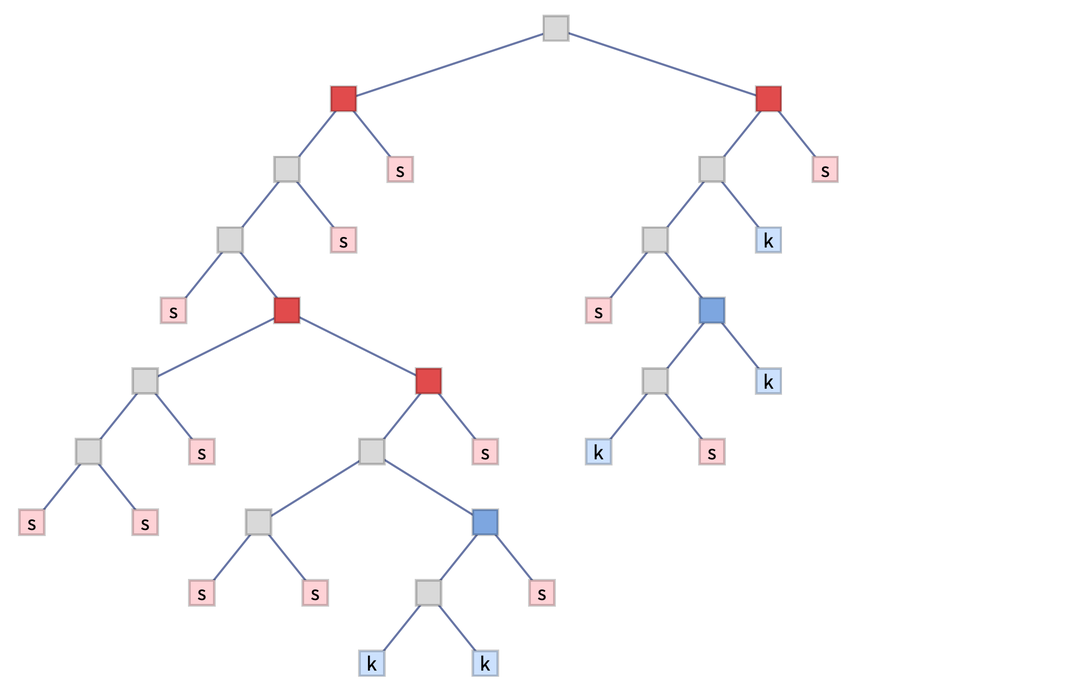
\includegraphics[width=12cm]{strategy}
  \captionsetup{justification=centering}
  \caption{Egy kombinátor absztrakt szintaxis fája. A különböző kiértékelési módok kiválóan bemutathatóak rajta.}
  \label{fig:strategy}
\end{figure}

\subsubsection{A \lam-kalkulus}
\label{sec:a-lam-kalkulus-impl}

A \lam-kalkulus kiértékelése bizonyos szempontból bonyolultabb, mint az \ski-kalkulusé. Ez részben abból adódik, hogy a \lam-kalkulusban vannak változók. Létezik viszont a \lam-kalkulusnak egy olyan alakja, amely -- bár teljesen nem tud megszabadulni tőlük -- egyszerűbbé teszi a kezelésüket. Ez az alak, a de Bruijn forma\footnote{Az általam használt változata a lokálisan névtelen de Bruijn forma}\cite{pierceTypesProgrammingLanguages2002a, chargueraudLocallyNamelessRepresentation2012b}. Ez a forma az úgynevezett de Bruijn indexeken alapul: egy \lam-kalkulus kifejezésben egy változó de Bruijn indexe az a szám, amely azt jelzi, hogy az őt "kötő" \lam-absztrakció hány szinttel van feljebb a kifejezés fájában. Például a \(\lam x.(\lam y. x)\) kifejezésben az \(x\) változó de Bruijn indexe \(2\), mivel az őt definiáló \lam-absztrakció (\(\lam x.\)) az két szinttel van feljebb. A kifejezés de Bruijn alakja tehát \(\lam\,\lam\,2\).

Az én \lam-kalkulus kiértékelőm ilyen alakban végzi el a kiértékelést, mivel így a kiértékelés során nem kell külön figyelni az úgynevezett \(\alpha\)-ekvivalenciára. Ehhez meg kellett valósítanom a konverziót a tradícionális \lam-kalkulus és a de Bruijn forma között mindkét irányban. Ezek után a de Bruijn alakra definiáltam a \(\beta\)-redukciót, amely megfelel egy \lam-absztrakció kiértékelésének egy változóval. Ez után definiáltam a különböző stratégiákat, amelyek csak abban térnek el, hogy a kifejezésben éppen melyik alkifejezést \(\beta\)-redukálják.

Három stratégiát valósítottam meg: \foreignlanguage{english}{normal order}, \foreignlanguage{english}{call--by--name} illetve \foreignlanguage{english}{call--by--value} \cite{Lambdakalkulus2007}. Azért erre a háromra esett a választás, mert szerettem volna mind \foreignlanguage{english}{lazy} és \foreignlanguage{english}{eager}, mind normálformára és nem-normálformára hozó stratégiákat elérhetővé tenni.

\subsection{Az \ski-kalkulus konverzió}
\label{sec:a-ski-kalkulus-konverzio}

Ahogy \aref{sec:a-ski-kalkulus-def}~fejezetben ismertettem, a konverzió az \ski-kalkulusból a \lam-kalkulusba egy triviális folyamat. Az egyes kombinátoroknak a definícióit behelyettesítve, meg is kaptam a konvertált \lam-kalkulus kifejezést. Az olvashatóság növelése érdekében az egyes változók mind-mind eltérő neveket kapnak (\(a\), \(b\), \dots, \(z\), \(a_1\), \(b_1\), \dots, \(z_1\), \(a_2\), \(b_2\), \dots, \(z_2\), \dots). A felhasználó a konverziót követően ki tudja másolni a konvertált \lam-kalkulus kifejezést. Az átváltást megfordítani -- azaz \lam-kalkulus kifejezéseket \ski-kalkulusra alakítani -- már közel sem ennyire triviális. Ez a \foreignlanguage{english}{bracket abstraction} (zárójel-absztrakció) témakörébe tartozik, melynek elméleti alapjait Moses Schönfinkel fektette le 1924-ben \cite{schoenfinkelUeberBausteineMathematischen1924}. Jelenleg nem létezik olyan optimális, lineáris algoritmus, amely tetszőleges \lam-kifejezést méretrobbanás nélkül tudna véges kombinátorbázisra (például \ski) lefordítani. Curry klasszikus absztrakciós algoritmusa \cite{curry1958combinatory} ugyan helyes, de használata során a kifejezések hossza drasztikusan, gyakran exponenciálisan megnőhet a kötött változók számának függvényében. Később David Turner ezt a folyamatot további kombinátorok bevezetésével optimalizálta, de a naiv eljárás legrosszabb esetben még így is legalább kvadratikus lépésigényű marad \cite{turner1979new}.


\subsection{A tesztelés}
\label{sec:a-teszt-orakulum-kialak}

A szoftver helyességének verifikálására a hagyományos egységtesztek mellett a \foreignlanguage{english}{Property-based testing} (tulajdonság-alapú tesztelés) módszertanát alkalmaztam. Ennek során a teszt-keretrendszer automatikusan generál valid, véletlenszerű \lam- és \ski-kifejezéseket, majd megvizsgálja a rendszer invariáns tulajdonságait.

A redukciós gépek kimenetének validálásához egy tesztelő orákulumot alakítottam ki \cite{howdenTheoreticalEmpiricalStudies1978}. Az orákulum egy már bizonyítottan helyesen működő, külső interpreter, amelyet egy elszigetelt Podman konténerben futtattam le a biztonság és a determinisztikus környezet garantálása érdekében. A tesztelési folyamat során a program és a Podman konténerben futó orákulum is kiértékelte ugyanazt a generált kifejezést, a teszt-keretrendszer pedig a két kimenet ekvivalenciáját vizsgálta \foreignlanguage{english}{Black-box} (fekete doboz) tesztelés formájában.

A fejlesztés folyamán a tesztelés által többször is hibás működésre lettem figyelmes, amit ki tudtam javítani. Az egyik ilyen az volt, amikor az \ski-kifejezések redukálása során, az indirekciós csúcsokat nem jól oldottam fel, és ez a redukciós folyamat egy későbbi fázisában (ahol már nem lett volna szabad indirekciós csúcsoknak lennie) hibához vezetett. Az indirekció feloldó algoritmus kijavítása után visszaállt a rendes működés. Egy másik eset során refaktoráltam a \lam-kalkulus kanonikus, és de Bruijn forma közötti átváltás folyamatát. A refaktorálás során egy olyan hiba került be, ami a backend teljes lefagyásához vezetett, amit csak a program újraindításával lehetett orvosolni. Ez abból fakadt, hogy véges számú nevesített változót támogattam csak a kanonikus alakban. Ezt a hibát egy egységteszt kiszűrte, ami után a jelenleg is használt, indexelt elnevezést implementáltam, így a hiba megszűnt.

\newpage

\subsection{A vizuális redukciós elemek létrehozása}
\label{sec:a-viz-reduk-elemek-letrehoz}

Egy oktatási eszköz esetében a belső folyamatok láthatósága kritikus jelentőségű, ezért a backendet felkészítettem arra, hogy úgynevezett \emph{\foreignlanguage{english}{callback}} függvényeket tudjon fogadni. Ezek a függvények egy olyan nézetet kapnak a belső gépről, amelyen olyan metódusok vannak definiálva, amelyekkel a teljes AST-t be lehet járni, szemantikai információt fűzve az egyes csúcsokhoz. Így az egyes redukciós lépések könnyen naplózhatóak, az alkifejezések különböző szerepe pedig elkülöníthető.

Algoritmusokat dolgoztam ki a redukálható kifejezések (redexek) detektálására és strukturált adatként (JSON) történő továbbítására a frontend felé. Ezek az adatok teszik lehetővé, hogy a webes felület vizuálisan kiemelje a soron következő redukciós lépést. Erre egy példa \aref{fig:visuals}.~ábrán látható. A különböző kombinátoroknak más-más színeik vannak, és meg vannak különböztetve a redukálható kifejezések az argumentumaiktól. \Aref{sec:a-redukcios-gepek-impl}~fejezetben tárgyalt részfamegosztás módszere miatt egyes kombinátorok többször is ki vannak színezve. Ez arra utal, hogy a kifejezés fájában az a látszólag két különböző kombinátor ugyan arra hivatkozik.

\begin{figure}[htbp]
  \centering
  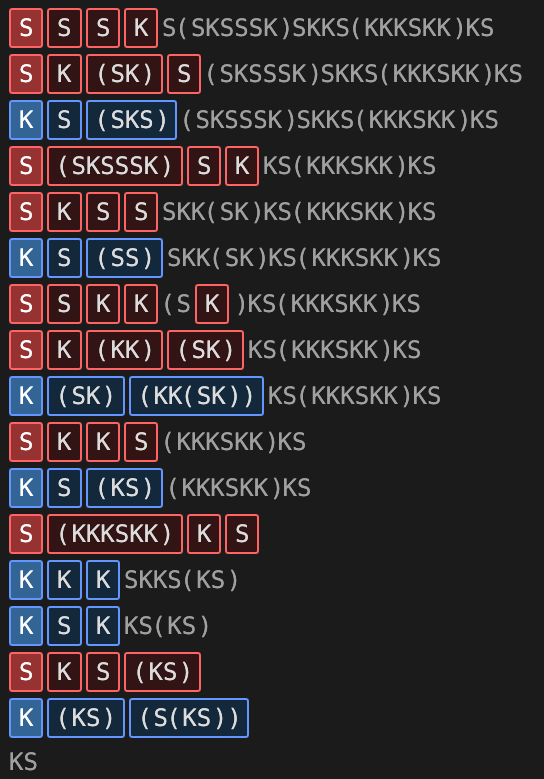
\includegraphics[width=8cm]{visuals}
  \captionsetup{justification=centering}
  \caption{Egy redukciós lánc, ahol az egyes kifejezések szemantikailag vannak kiszínezve.}
  \label{fig:visuals}
\end{figure}

A redukciós láncon kívül a kifejezések gráfként való reprezentálását is implementálnom kellett. Az algoritmus aktuális gráfállapot kinyeréséhez a \foreignlanguage{english}{G-machine} memóriájában lévő gyökérelemből kiindulva egy mélységi bejárást (\foreignlanguage{english}{Depth-First Search}) végez. A bejáró algoritmus külön kezeli a redukció során keletkező indirekciós csomópontokat: ezeket transzparens módon feloldja, és addig követi a mutatókat, amíg egy tényleges applikációt vagy kombinátort nem ér el. A végeredményt a \foreignlanguage{english}{G-machine} egy lapos listává alakítja. Ebben a listában minden csomópont tartalmazza a típusát (\texttt{App} vagy \texttt{Comb}), a gyermekei azonosítóinak tömbjét, valamint a saját egyedi azonosítóját, amelyet közvetlenül az aréna belső mutatóiból származtatok. Ez a mutatómentes, lapos reprezentáció optimális a JSON-szerializációhoz és a WebAssembly határon történő gyors átvitelhez, amely alapján a frontend  keretrendszere képes felépíteni a vizuális gráfot.

\subsection{A frontend fejlesztése}
\label{sec:a-frontend-fejl}

A frontend egy teljes mértékben kliensoldalon futó alkalmazás, amelyet Rust nyelvből WebAssembly-re (WASM) fordítottam.

Az Elm-architektúrára épülő reaktív felületen a felhasználó interaktívan gépelhet be kifejezéseket, kiválaszthatja a kívánt kalkulust és a kiértékelési stratégiát. A gördülékeny felhasználói élmény érdekében a háttérfolyamatokat Service Worker-ekbe (\texttt{worker.js}) szerveztem. Így a komplex és esetlegesen hosszú ideig futó redukciós fák kiértékelése nem fagyasztja le a felhasználói felületet, és a szoftver akár offline módban (PWA) is képes teljeskörűen funkcionálni. A grafikus felületet \aref{fig:ui}.~ábrán mutatom be.

Az egui \cite{egui} grafikus keretrendszert használtam a felület kialakítására, amely egy úgynevezett \emph{\foreignlanguage{english}{immediate mode}} grafikus felület. Ennek a megközelítésnek az a különlegessége, hogy a felhasználói felület minden egyes képkockánál a nulláról épül fel és rajzolódik ki. A gombok, vagy beviteli mezők állapota nincsen eltárolva a memóriában két egymást követő \foreignlanguage{english}{frame} között. Ez azt is jelenti, hogy a felület kirajzolása, és a felhasználói interakciók kezelése egyetlen lépésben történik.

\begin{figure}[htbp]
  \centering
  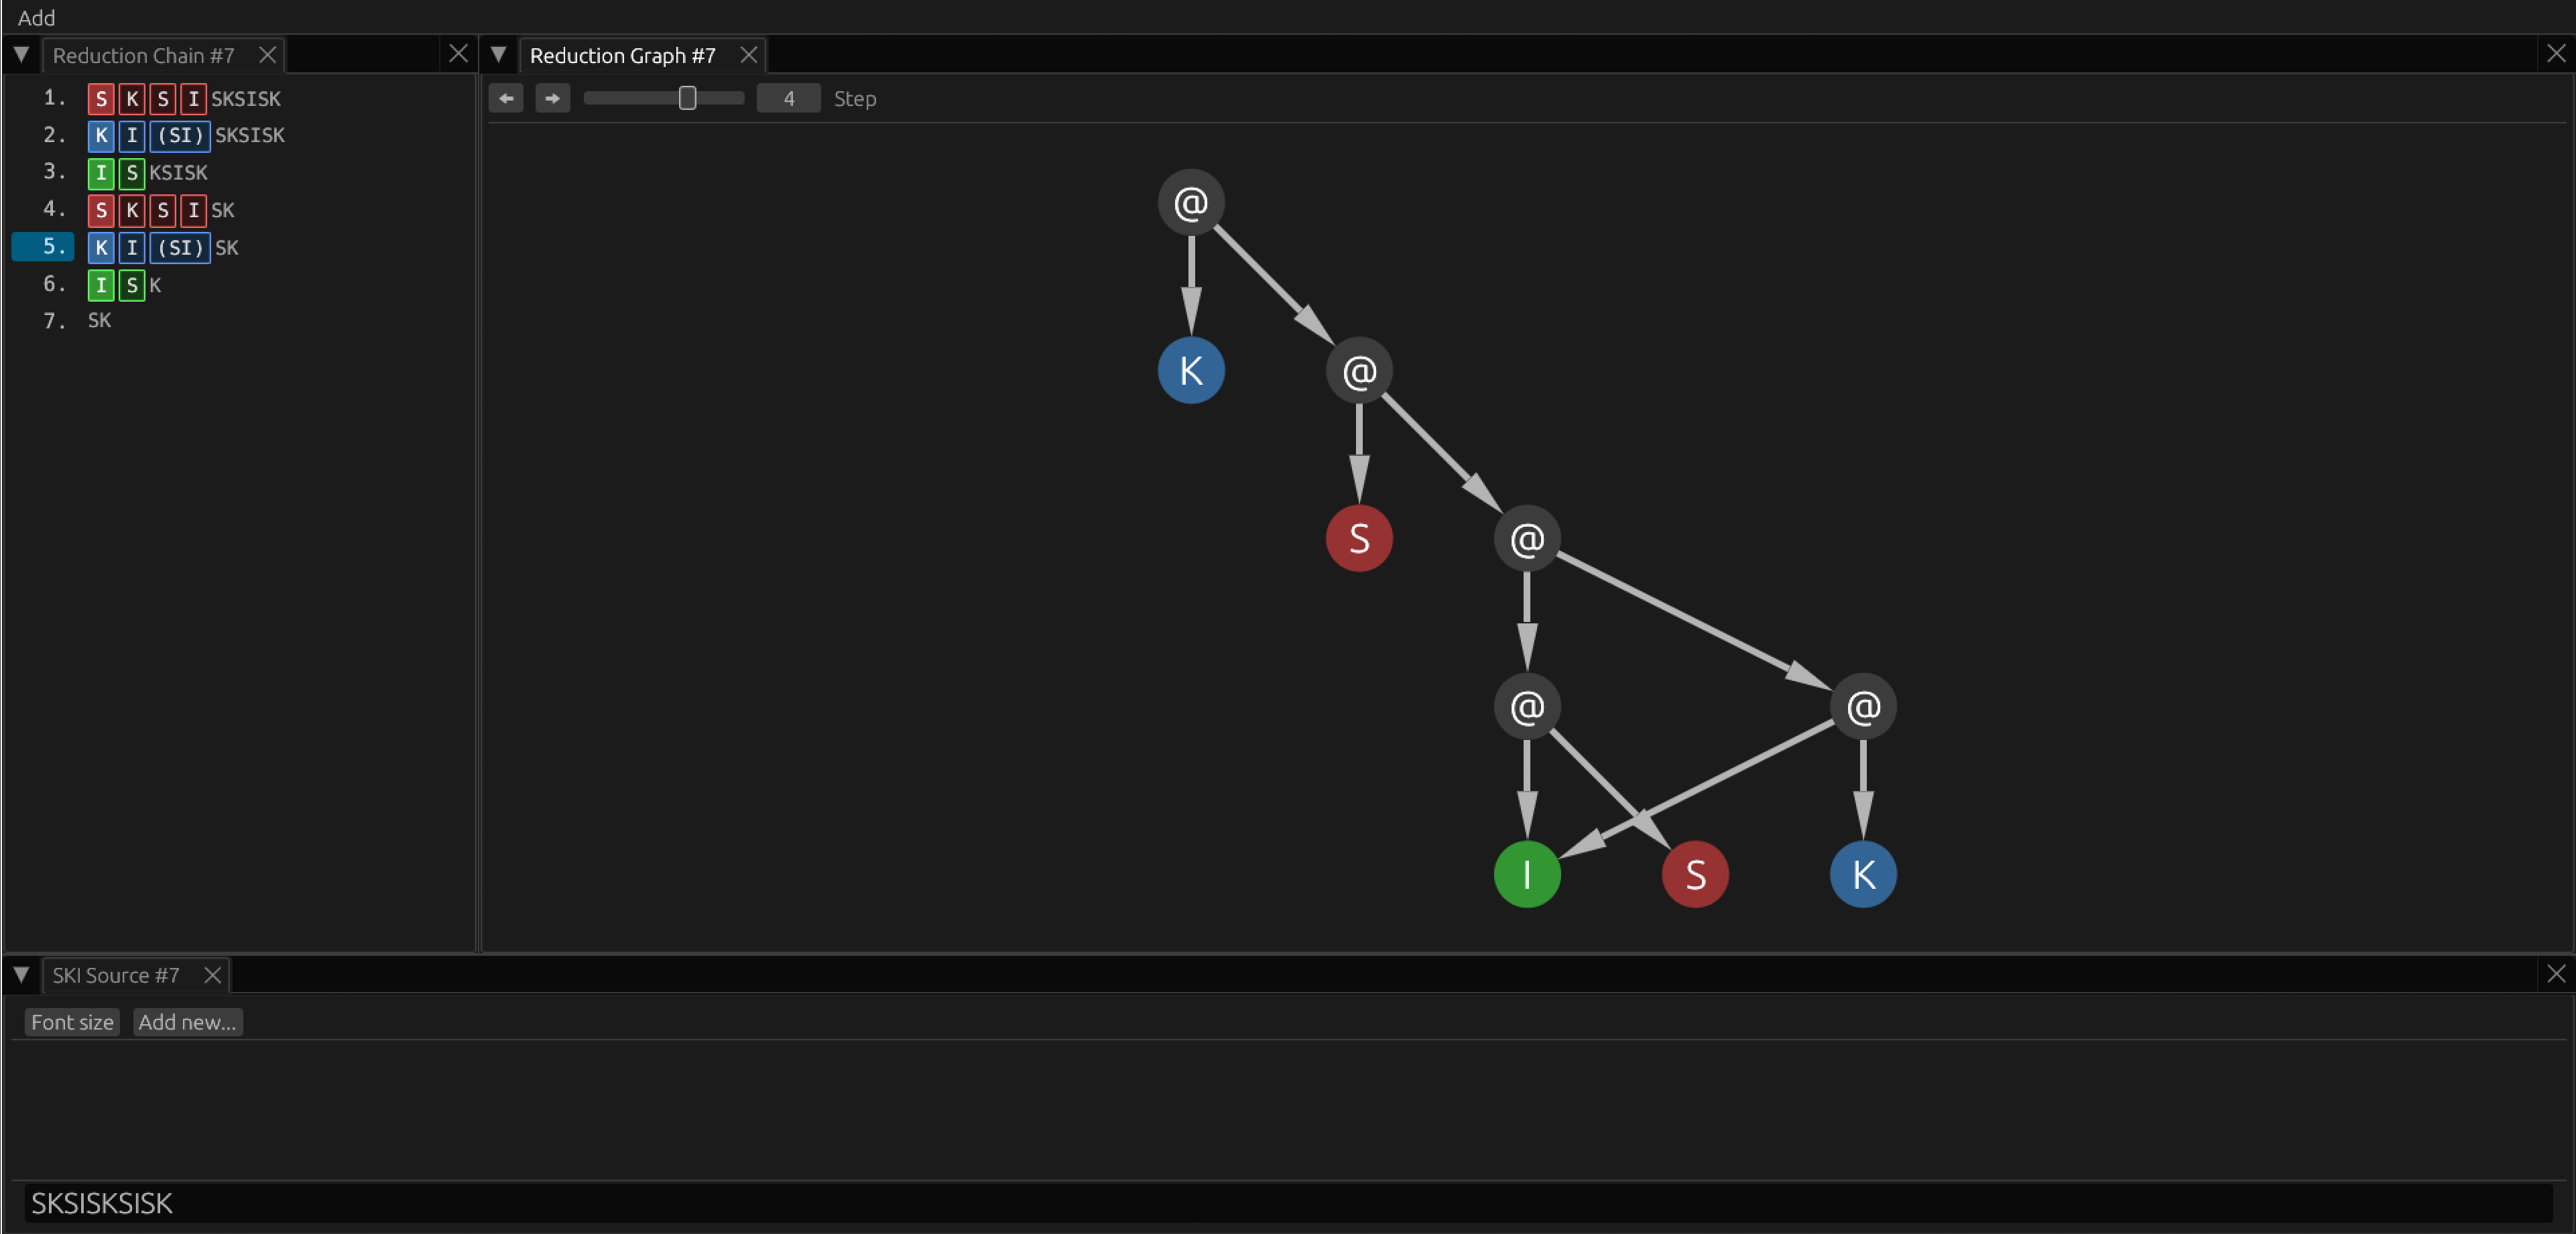
\includegraphics[width=15cm]{ui}
  \captionsetup{justification=centering}
  \caption{A grafikus felülete a programnak. A jobb felső sarokban egy redukciós lánc látható. A bal felső sarokban egy \ski-kalkulus bemeneti ablak van, ahol megjelenik a megadott kifejezés \lam-kalkulusba konvertált alakja is. A bal alsó sarokban egy \lam-kalkulus bemenető ablak helyezkedik el. Végezetül a jobb alsó sarokban a megadott \ski-kalkulus kifejezéshez tartozó redukciós gráf egyik lépése látható.}
  \label{fig:ui}
\end{figure}

\subsection{Elérhetőség}
\label{sec:elerhetoseg}

A projekt elérhető GitHubon. A telepítési útmutató, futtatási utasítások és forráskód szabadon megtekinthetőek\cite{levyLevyryLexor2026}.

\subsection{Összefoglalás}
\label{sec:osszefoglalas}

A félév során sikeresen megvalósítottam a munkatervben kitűzött célokat. Áttanulmányoztam a releváns szakirodalmat, ami alapján megterveztem az architektúrát. Kialakítottam a nyelvtanokat feldolgozó parsereket, implementáltam mind a \lam-, mind az \ski-kalkulus G-machine alapú redukciós gépét, és mindezt egy WebAssembly alapú, interaktív frontenddel kötöttem össze. A Podman konténeres orákulumra épülő \foreignlanguage{english}{Property-based testing} gondoskodik a motorok megbízhatóságáról. Az elkészült \emph{Combinator Explorer} eszköz így sikeresen tölti be funkcióját: vizuális formát ad a funkcionális programozás matematikai alapjainak, hatékony és korszerű segédeszközt nyújtva a felsőoktatás számára.

\newpage

%==================================================================
\section{Irodalom, és csatlakozó dokumentumok jegyzéke}
\label{sec:irod-es-csatl}

\label{sec:tanulm-irod-jegyz}
\bibliographystyle{huplain}
\bibliography{irodalom}
%==================================================================

\end{document}

%%% Local Variables: 
%%% mode: latex 
%%% TeX-master: t 
%%% End:

